\documentclass{ximera}

 

\usepackage{epsfig}

\graphicspath{
  {./}
  {figures/}
}

\usepackage{morewrites}
\makeatletter
\newcommand\subfile[1]{%
\renewcommand{\input}[1]{}%
\begingroup\skip@preamble\otherinput{#1}\endgroup\par\vspace{\topsep}
\let\input\otherinput}
\makeatother

\newcommand{\includeexercises}{\directlua{dofile("/home/jim/linearAlgebra/laode/exercises.lua")}}

%\newcounter{ccounter}
%\setcounter{ccounter}{1}
%\newcommand{\Chapter}[1]{\setcounter{chapter}{\arabic{ccounter}}\chapter{#1}\addtocounter{ccounter}{1}}

%\newcommand{\section}[1]{\section{#1}\setcounter{thm}{0}\setcounter{equation}{0}}

%\renewcommand{\theequation}{\arabic{chapter}.\arabic{section}.\arabic{equation}}
%\renewcommand{\thefigure}{\arabic{chapter}.\arabic{figure}}
%\renewcommand{\thetable}{\arabic{chapter}.\arabic{table}}

%\newcommand{\Sec}[2]{\section{#1}\markright{\arabic{ccounter}.\arabic{section}.#2}\setcounter{equation}{0}\setcounter{thm}{0}\setcounter{figure}{0}}

\newcommand{\Sec}[2]{\section{#1}}

\setcounter{secnumdepth}{2}
%\setcounter{secnumdepth}{1} 

%\newcounter{THM}
%\renewcommand{\theTHM}{\arabic{chapter}.\arabic{section}}

\newcommand{\trademark}{{R\!\!\!\!\!\bigcirc}}
%\newtheorem{exercise}{}

\newcommand{\dfield}{{\sf dfield9}}
\newcommand{\pplane}{{\sf pplane9}}

\newcommand{\EXER}{\section*{Exercises}}%\vspace*{0.2in}\hrule\small\setcounter{exercise}{0}}
\newcommand{\CEXER}{}%\vspace{0.08in}\begin{center}Computer Exercises\end{center}}
\newcommand{\TEXER}{} %\vspace{0.08in}\begin{center}Hand Exercises\end{center}}
\newcommand{\AEXER}{} %\vspace{0.08in}\begin{center}Hand Exercises\end{center}}

% BADBAD: \newcommand{\Bbb}{\bf}

\newcommand{\R}{\mbox{$\Bbb{R}$}}
\newcommand{\C}{\mbox{$\Bbb{C}$}}
\newcommand{\Z}{\mbox{$\Bbb{Z}$}}
\newcommand{\N}{\mbox{$\Bbb{N}$}}
\newcommand{\D}{\mbox{{\bf D}}}
\usepackage{amssymb}
%\newcommand{\qed}{\hfill\mbox{\raggedright$\square$} \vspace{1ex}}
%\newcommand{\proof}{\noindent {\bf Proof:} \hspace{0.1in}}

\newcommand{\setmin}{\;\mbox{--}\;}
\newcommand{\Matlab}{{M\small{AT\-LAB}} }
\newcommand{\Matlabp}{{M\small{AT\-LAB}}}
\newcommand{\computer}{\Matlab Instructions}
\newcommand{\half}{\mbox{$\frac{1}{2}$}}
\newcommand{\compose}{\raisebox{.15ex}{\mbox{{\scriptsize$\circ$}}}}
\newcommand{\AND}{\quad\mbox{and}\quad}
\newcommand{\vect}[2]{\left(\begin{array}{c} #1_1 \\ \vdots \\
 #1_{#2}\end{array}\right)}
\newcommand{\mattwo}[4]{\left(\begin{array}{rr} #1 & #2\\ #3
&#4\end{array}\right)}
\newcommand{\mattwoc}[4]{\left(\begin{array}{cc} #1 & #2\\ #3
&#4\end{array}\right)}
\newcommand{\vectwo}[2]{\left(\begin{array}{r} #1 \\ #2\end{array}\right)}
\newcommand{\vectwoc}[2]{\left(\begin{array}{c} #1 \\ #2\end{array}\right)}

\newcommand{\ignore}[1]{}


\newcommand{\inv}{^{-1}}
\newcommand{\CC}{{\cal C}}
\newcommand{\CCone}{\CC^1}
\newcommand{\Span}{{\rm span}}
\newcommand{\rank}{{\rm rank}}
\newcommand{\trace}{{\rm tr}}
\newcommand{\RE}{{\rm Re}}
\newcommand{\IM}{{\rm Im}}
\newcommand{\nulls}{{\rm null\;space}}

\newcommand{\dps}{\displaystyle}
\newcommand{\arraystart}{\renewcommand{\arraystretch}{1.8}}
\newcommand{\arrayfinish}{\renewcommand{\arraystretch}{1.2}}
\newcommand{\Start}[1]{\vspace{0.08in}\noindent {\bf Section~\ref{#1}}}
\newcommand{\exer}[1]{\noindent {\bf \ref{#1}}}
\newcommand{\ans}{}
\newcommand{\matthree}[9]{\left(\begin{array}{rrr} #1 & #2 & #3 \\ #4 & #5 & #6
\\ #7 & #8 & #9\end{array}\right)}
\newcommand{\cvectwo}[2]{\left(\begin{array}{c} #1 \\ #2\end{array}\right)}
\newcommand{\cmatthree}[9]{\left(\begin{array}{ccc} #1 & #2 & #3 \\ #4 & #5 &
#6 \\ #7 & #8 & #9\end{array}\right)}
\newcommand{\vecthree}[3]{\left(\begin{array}{r} #1 \\ #2 \\
#3\end{array}\right)}
\newcommand{\cvecthree}[3]{\left(\begin{array}{c} #1 \\ #2 \\
#3\end{array}\right)}
\newcommand{\cmattwo}[4]{\left(\begin{array}{cc} #1 & #2\\ #3
&#4\end{array}\right)}

\newcommand{\Matrix}[1]{\ensuremath{\left(\begin{array}{rrrrrrrrrrrrrrrrrr} #1 \end{array}\right)}}

\newcommand{\Matrixc}[1]{\ensuremath{\left(\begin{array}{cccccccccccc} #1 \end{array}\right)}}



\renewcommand{\labelenumi}{\theenumi)}
\newenvironment{enumeratea}%
{\begingroup
 \renewcommand{\theenumi}{\alph{enumi}}
 \renewcommand{\labelenumi}{(\theenumi)}
 \begin{enumerate}}
 {\end{enumerate}\endgroup}



\newcounter{help}
\renewcommand{\thehelp}{\thesection.\arabic{equation}}

%\newenvironment{equation*}%
%{\renewcommand\endequation{\eqno (\theequation)* $$}%
%   \begin{equation}}%
%   {\end{equation}\renewcommand\endequation{\eqno \@eqnnum
%$$\global\@ignoretrue}}

%\input{psfig.tex}

\author{Martin Golubitsky and Michael Dellnitz}

%\newenvironment{matlabEquation}%
%{\renewcommand\endequation{\eqno (\theequation*) $$}%
%   \begin{equation}}%
%   {\end{equation}\renewcommand\endequation{\eqno \@eqnnum
% $$\global\@ignoretrue}}

\newcommand{\soln}{\textbf{Solution:} }
\newcommand{\exercap}[1]{\centerline{Figure~\ref{#1}}}
\newcommand{\exercaptwo}[1]{\centerline{Figure~\ref{#1}a\hspace{2.1in}
Figure~\ref{#1}b}}
\newcommand{\exercapthree}[1]{\centerline{Figure~\ref{#1}a\hspace{1.2in}
Figure~\ref{#1}b\hspace{1.2in}Figure~\ref{#1}c}}
\newcommand{\para}{\hspace{0.4in}}

\renewenvironment{solution}{\suppress}{\endsuppress}

\ifxake
\newenvironment{matlabEquation}{\begin{equation}}{\end{equation}}
\else
\newenvironment{matlabEquation}%
{\let\oldtheequation\theequation\renewcommand{\theequation}{\oldtheequation*}\begin{equation}}%
  {\end{equation}\let\theequation\oldtheequation}
\fi

\makeatother


\title{c9.tex}

\begin{document}
\begin{abstract}
BADBAD
\end{abstract}
\maketitle

\chapter{Linear Maps and Changes of Coordinates}
\label{C:LMCC}

\normalsize

The first section in this chapter, Section~\ref{Sect:linmap}, defines linear 
mappings between abstract vector spaces, shows how such mappings are
determined by their values on a basis, and derives basic properties of 
invertible linear mappings. 
  
The notions of {\em row rank\/} and {\em column rank\/} of a matrix are
discussed in Section~\ref{S:5.8} along with the theorem that states that
these numbers are equal to the rank of that matrix.

Section~\ref{S:coordinates} discusses the underlying meaning of similarity 
--- the different ways to view the same linear mapping on $\R^n$ in different 
coordinates systems or bases.  This discussion makes sense only after the 
definitions of coordinates corresponding to bases and of changes in 
coordinates are given and justified.  In Section~\ref{MALT}, we discuss the 
matrix associated to a linearity transformation between two finite
dimensional vector spaces in a given set of coordinates and show that changes 
in coordinates correspond to similarity of the corresponding matrices.



\section{Linear Mappings and Bases}  \label{Sect:linmap}

The examples of linear mappings
\index{linear!mapping} from $\R^n\to\R^m$ that we introduced in
Section~\ref{S:linearity} were matrix mappings.  More precisely,
let $A$ be an $m\times n$ matrix.  Then
\[
L_A(x)=Ax
\]
defines the linear mapping $L_A:\R^n\to\R^m$.  Recall that $Ae_j$
is the $j^{th}$ column of $A$ (see Chapter~\ref{chap:matrices},
Lemma~\ref{columnsA}); it follows that $A$ can be
reconstructed from the vectors $Ae_1,\ldots,Ae_n$.  This remark
implies (Chapter~\ref{chap:matrices}, Lemma~\ref{linequal}) that
linear mappings of $\R^n$ to $\R^m$ are determined by their
values on the standard basis $e_1, \ldots, e_n$.  Next we show
that this result is valid in greater generality.  We begin by
defining what we mean for a mapping between vector spaces to be
linear.

\begin{Def}  \label{D:linearV}
Let $V$ and $W$ be vector spaces and let $L:V\to W$ be a mapping.  The map
$L$ is {\em linear\/} if
\begin{eqnarray*}
L(u+v) & = & L(u) + L(v) \\
L(cv) & = & cL(v)
\end{eqnarray*}
for all $u,v\in V$ and $c\in\R$.
\end{Def} \index{linear}\index{vector!space}

\subsubsection*{Examples of Linear Mappings}

\noindent (a) Let $v\in\R^n$ be a fixed vector.  Use the
dot product\index{dot product} to define the mapping
$L:\R^n\to\R$ by
\[
L(x)= x\cdot v.
\]
Then $L$ is linear.  Just check that
\[
L(x+y) = (x+y)\cdot v = x\cdot v + y\cdot v = L(x) + L(y)
\]
for every vector $x$ and $y$ in $\R^n$ and
\[
L(cx) = (cx)\cdot v = c(x\cdot v) = cL(x)
\]
for every scalar $c\in\R$.

\noindent (b) The map $L:\CCone\to\R$ defined by
\[
L(f) = f'(2)
\]
is linear.  Indeed,
\[
L(f+g) = (f+g)'(2) = f'(2) + g'(2) = L(f) + L(g).
\]
Similarly, $L(cf)=cL(f)$.

\noindent (c) The map $L:\CCone\to\CCone$ defined by
\[
L(f)(t)=f(t-1)
\]
is linear.  Indeed,
\[
L(f+g)(t) = (f+g)(t-1) = f(t-1) + g(t-1) = L(f)(t) + L(g)(t).
\]
Similarly, $L(cf)=cL(f)$.  It may be helpful to compute $L(f)(t)$ when
$f(t)=t^2-t+1$.  That is,
\[
L(f)(t) = (t-1)^2-(t-1)+1 = t^2-2t+1-t+1+1 = t^2-3t+3.
\]


\subsubsection*{Constructing Linear Mappings from Bases}

\begin{thm} \label{L:linmapfrombasis}
Let $V$ and $W$ be vector spaces.  Let $\{v_1,\ldots,v_n\}$ be a
basis for $V$ and let $\{w_1,\ldots,w_n\}$ be $n$ vectors in $W$.
Then there exists a unique linear map $L:V\to W$ such that $L(v_i)=w_i$.
\end{thm}\index{linear!mapping!construction}

\begin{proof} Let $v\in V$ be a vector.  Since $\Span\{v_1,\ldots,v_n\}=V$, we may
write $v$ as
\[
v = \alpha_1v_1 + \cdots + \alpha_nv_n,
\]
where $\alpha_1,\ldots,\alpha_n$ in $\R$.   Moreover, $v_1,\ldots,v_n$
are linearly independent, these scalars are uniquely defined.  More
precisely, if
\[
\alpha_1v_1 + \cdots + \alpha_nv_n = \beta_1v_1 + \cdots + \beta_nv_n,
\]
then
\[
(\alpha_1-\beta_1)v_1 + \cdots + (\alpha_n-\beta_n)v_n = 0.
\]
Linear independence implies that $\alpha_j-\beta_j=0$; that is
$\alpha_j=\beta_j$.   We can now define
\begin{equation}  \label{e:v-coord}
L(v) = \alpha_1 w_1+\cdots+\alpha_n w_n.
\end{equation}

We claim that $L$ is linear.  Let $\hat{v}\in V$ be another
vector and let
\[
\hat{v} = \beta_1v_1+\cdots+\beta_nv_n.
\]
It follows that
\[
v+\hat{v} = (\alpha_1+\beta_1)v_1+\cdots+(\alpha_n+\beta_n)v_n,
\]
and hence by \Ref{e:v-coord} that
\begin{eqnarray*}
L(v+\hat{v}) & = &
(\alpha_1+\beta_1)w_1+\cdots+(\alpha_n+\beta_n)w_n\\
& = & (\alpha_1w_1+\cdots+\alpha_nw_n) +
(\beta_1w_1+\cdots+\beta_nw_n)  \\
& = & L(v) + L(\hat{v}).
\end{eqnarray*}

Similarly
\begin{eqnarray*}
L(cv) &  = & L( (c\alpha_1)v_1+\cdots +(c\alpha_n)v_n)\\
& = & c(\alpha_1w_1+\cdots+\alpha_nw_n)\\
& = & cL(v).
\end{eqnarray*}
Thus $L$ is linear.

Let $M:V\to W$ be another linear mapping such that $M(v_i)=w_i$.
Then
\begin{eqnarray*}
L(v) & = & L(\alpha_1v_1+\ldots +\alpha_nv_n)\\
& = & \alpha_1w_1+\cdots+\alpha_nw_n \\
& = & \alpha_1M(v_1) + \cdots +\alpha_nM(v_n)\\
& = & M(\alpha_1v_1 + \cdots +\alpha_nv_n)\\
& = & M(v).
\end{eqnarray*}
Thus $L=M$ and the linear mapping is uniquely defined.  \end{proof}


There are two assertions made in Theorem~\ref{L:linmapfrombasis}.
The first is that a linear map exists mapping $v_i$ to $w_i$.
The second is that there is only one {\em linear\/} mapping
that accomplishes this task.  If we drop the constraint that the
map be linear, then many mappings may satisfy these conditions.
For example, find a linear map from $\R\to\R$ that maps $1$ to $4$.
There is only one: $y=4x$.  However there are many nonlinear maps
that send $1$ to $4$.  Examples are $y=x+3$ and $y=4x^2$.

\subsubsection*{Finding the Matrix of a Linear Map from $\R^n\to\R^m$
Given by Theorem~\protect{\ref{L:linmapfrombasis}}}
\index{linear!mapping!matrix}

Suppose that $V=\R^n$ and $W=\R^m$.  We know that every linear
map $L:\R^n\to\R^m$ can be defined as multiplication by an
$m\times n$ matrix.  The question that we next address is:
How can we find the matrix whose existence is guaranteed by
Theorem~\ref{L:linmapfrombasis}?

More precisely, let $v_1,\ldots,v_n$ be a basis for $\R^n$ and
let $w_1,\ldots,w_n$ be vectors in $\R^m$.  We suppose that all
of these vectors are row vectors.  Then we need to find
an $m\times n$ matrix $A$ such that $Av_i^t=w_i^t$ for all $i$.
We find $A$ as follows.  Let $v\in\R^n$ be a row vector.  Since
the $v_i$ form a basis, there exist scalars $\alpha_i$ such that
\[
v=\alpha_1 v_1 + \cdots + \alpha_n v_n.
\]
In coordinates
\begin{equation}  \label{e:v^t}
v^t = (v_1^t|\cdots|v_n^t)\vect{\alpha}{n},
\end{equation}
where $(v_1^t|\cdots|v_n^t)$ is an $n\times n$
invertible matrix\index{matrix!invertible}.
By definition (see \Ref{e:v-coord})
\[
L(v) = \alpha_1 w_1 + \cdots + \alpha_n w_n.
\]
Thus the matrix $A$ must satisfy
\[
Av^t = (w_1^t|\cdots|w_n^t)\vect{\alpha}{n},
\]
where $(w_1^t|\cdots|w_n^t)$ is an $m\times n$ matrix.
Using \Ref{e:v^t} we see that
\[
Av^t = (w_1^t|\cdots|w_n^t)(v_1^t|\cdots|v_n^t)\inv v^t,
\]
and
\begin{equation}  \label{e:defA}
A = (w_1^t|\cdots|w_n^t)(v_1^t|\cdots|v_n^t)\inv
\end{equation}
is the desired $m\times n$ matrix.

\subsubsection*{An Example of a Linear Map from $\R^3$ to $\R^2$}

As an example we illustrate Theorem~\ref{L:linmapfrombasis} and
\Ref{e:defA} by defining a linear mapping from $\R^3$ to $\R^2$
by its action on a basis.  Let
\[
v_1=(1,4,1)\quad v_2=(-1,1,1) \quad v_3=(0,1,0).
\]
We claim that $\{v_1,v_2,v_3\}$ is a basis of $\R^3$ and that
there is a unique linear map for which $L(v_i)=w_i$ where
\[
w_1=(2,0) \quad w_2=(1,1) \quad w_3=(1,-1).
\]

We can verify that $\{v_1,v_2,v_3\}$ is a basis of $\R^3$ by
showing that the matrix
\[
(v_1^t|v_2^t|v_3^t) = \left(\begin{array}{rrr}
1 & -1 & 0  \\
4 & 1 & 1  \\
1 & 1 & 0  \end{array}\right)
\]
is invertible.  This can either be done in \Matlab using the
{\tt inv} command or by hand by row reducing the matrix

\[
\left(\begin{array}{rrr|ccc}
1 & -1 & 0 & 1 & 0 & 0 \\
4 &  1 & 1 & 0 & 1 & 0 \\
1 &  1 & 0 & 0 & 0 & 1  \end{array}\right)
\]
to obtain
\[
(v_1^t|v_2^t|v_3^t)\inv = \frac{1}{2}\left(\begin{array}{rrr}
 1 & 0 &  1 \\
-1 & 0 &  1 \\
-3 & 2 & -5
\end{array}\right).
\]
Now apply \Ref{e:defA} to obtain
\[
A = \frac{1}{2} \left(\begin{array}{rrr} 2 & 1 & 1\\ 0 & 1 & -1
\end{array}\right) \left(\begin{array}{rrr}
 1 & 0 &  1 \\
-1 & 0 &  1 \\
-3 & 2 & -5
\end{array}\right) = \left(\begin{array}{rrr} -1 & 1 & -1 \\ 1 & -1 & 3
\end{array}\right).
\]
As a check, verify by matrix multiplication that $Av_i=w_i$, as claimed.


\subsection*{Properties of Linear Mappings}

\begin{lemma} \label{L:compose}
Let $U,V,W$ be vector spaces and $L:V\to W$ and $M:U\to V$ be linear maps.
Then $L\compose M :U\to W$ is linear.
\end{lemma}\index{composition!of linear mappings}

\begin{proof} The proof of Lemma~\ref{L:compose} is identical to that of
Chapter~\ref{chap:matrices}, Lemma~\ref{complin}. \end{proof}

A linear map $L:V\to W$ is {\em invertible\/} \index{invertible} if there
exists a linear map $M:W\to V$ such that $L\compose M:W\to W$ is the identity
map on $W$ and $M\compose L:V\to V$ is the identity map on $V$.

\begin{thm} \label{T:invertbasis}
Let $V$ and $W$ be finite dimensional vector spaces and let $v_1,\ldots,v_n$
be a basis\index{basis} for $V$.  Let $L:V\to W$ be a linear map.
Then $L$ is invertible
if and only if $w_1,\ldots,w_n$ is a basis for $W$ where $w_j=L(v_j)$.
\end{thm}

\begin{proof}  If $w_1,\ldots,w_n$ is a basis for $W$, then use
Theorem~\ref{L:linmapfrombasis} to define a linear map $M:W\to V$ by
$M(w_j)=v_j$.  Note that
\[
L\compose M(w_j)= L(v_j) =w_j.
\]
It follows by linearity (using the uniqueness part of
Theorem~\ref{L:linmapfrombasis}) that $L\compose M$ is the identity of $W$.
Similarly, $M\compose L$ is the identity map on $V$, and $L$ is invertible.

Conversely, suppose that $L\compose M$ and $M\compose L$ are identity maps
and that $w_j=L(v_j)$.  We must show that $w_1,\ldots,w_n$ is a basis.  We
use Theorem~\ref{basis=span+indep} and verify separately that
$w_1,\ldots,w_n$ are linearly independent and span $W$.

If there exist scalars $\alpha_1,\ldots,\alpha_n$ such that
\[
\alpha_1w_1+\cdots +\alpha_nw_n = 0,
\]
then apply $M$ to both sides of this equation to obtain
\[
0=M(\alpha_1w_1+\cdots +\alpha_nw_n)=\alpha_1v_1+\cdots+\alpha_nv_n.
\]
But the $v_j$ are linearly independent.  Therefore, $\alpha_j=0$ and the
$w_j$ are linearly independent.

To show that the $w_j$ span $W$, let $w$ be a vector in $W$.  Since the $v_j$
are a basis for $V$, there exist scalars $\beta_1,\ldots,\beta_n$ such that
\[
M(w) = \beta_1v_1+\cdots+\beta_nv_n.
\]
Applying $L$ to both sides of this equation yields
\[
w = L\compose M(w) = \beta_1w_1+\cdots+\beta_nw_n.
\]
Therefore, the $w_j$ span $W$.  \end{proof}

\begin{cor}
Let $V$ and $W$ be finite dimensional vector spaces.  Then there exists
an invertible\index{invertible} linear map $L:V\to W$
if and only if $\dim(V)=\dim(W)$.
\end{cor}

\begin{proof}  Suppose that $L:V\to W$ is an invertible linear map.  Let
$v_1,\ldots,v_n$ be a basis for $V$ where $n=\dim(V)$.  Then
Theorem~\ref{T:invertbasis} implies that $L(v_1),\ldots,L(v_n)$ is a basis
for $W$ and $\dim(W)=n=\dim(V)$.

Conversely, suppose that $\dim(V)=\dim(W)=n$.  Let $v_1,\ldots,v_n$ be a
basis for $V$ and let $w_1,\ldots,w_n$ be a basis for $W$.  Using
Theorem~\ref{L:linmapfrombasis} define the linear map $L:V\to W$ by
$L(v_j)=w_j$.  Theorem~\ref{T:invertbasis} states that $L$ is invertible. \end{proof}

\EXER

\TEXER

\begin{exercise} \label{c7.2.1}
Use the method described above to construct a linear mapping $L$
from $\R^3$ to $\R^2$ with $L(v_i)=w_i$, $i=1,2,3$, where
\[
v_1=(1,0,2)\quad v_2=(2,-1,1) \quad v_3=(-2,1,0)
\]
and
\[
w_1=(-1,0) \quad w_2=(0,1) \quad w_3=(3,1).
\]
\end{exercise}

\begin{exercise}  \label{c7.2.2}
Let ${\cal P}_n$ be the vector space of polynomials $p(t)$ of
degree less than or equal to $n$.  Show that $\{1,t,t^2,\ldots,t^n\}$ is a
basis for ${\cal P}_n$.
\end{exercise}

\begin{exercise}  \label{c7.2.2a}
Show that
\[
\frac{d}{dt}:{\cal P}_3\to{\cal P}_2
\]
is a linear mapping.
\end{exercise}
\begin{exercise}  \label{c7.2.2b}
Show that
\[
L(p) = \int_0^tp(s)ds
\]
is a linear mapping of ${\cal P}_2\to{\cal P}_3$.
\end{exercise}
\begin{exercise}  \label{c7.2.2c}
Use Exercises~\ref{c7.2.2a}, \ref{c7.2.2b} and
Theorem~\ref{L:linmapfrombasis} to show that
\[
\frac{d}{dt}\compose L:{\cal P}_2\to{\cal P}_2
\]
is the identity map.
\end{exercise}

\begin{exercise} \label{c7.2.3}
Let $\C$ denote the set of complex numbers.  Verify that
$\C$ is a two-dimensional vector space.  Show that $L:\C\to\C$
defined by
\[
L(z) = \lambda z,
\]
where $\lambda=\sigma+i\tau$ is a linear mapping.
\end{exercise}

\begin{exercise} \label{c7.2.4}
Let ${\cal M}(n)$ denote the vector space of $n\times n$
matrices and let $A$ be an $n\times n$ matrix.  Let
$L:{\cal M}(n)\to{\cal M}(n)$ be the mapping defined by
$L(X)=AX-XA$ where $X\in{\cal M}(n)$.  Verify that $L$ is
a linear mapping.  Show that the null space of $L$,
$\{X\in{\cal M}:L(X)=0\}$, is a subspace consisting of all
matrices that commute with $A$.
\end{exercise}

\begin{exercise} \label{c7.2.5}
Let $L:\CCone\to\R$ be defined by $L(f) = \int_0^{2\pi}f(t)\cos(t)dt$
for $f\in\CCone$.  Verify that $L$ is a linear mapping.
\end{exercise}

\begin{exercise} \label{c7.2.6}
Let ${\cal P}$ be the vector space of polynomials in one variable
$x$.  Define $L:{\cal P}\to {\cal P}$ by $L(p)(x)=\int_0^x(t-1)p(t)dt$.
Verify that $L$ is a linear mapping.
\end{exercise}


\section{Row Rank Equals Column Rank} \label{S:5.8}

Let $A$ be an $m\times n$ matrix.  The {\em row space\/}
\index{row!space} of $A$ is the span of the row vectors of $A$
and is a subspace of $\R^n$.  The {\em column space\/}
\index{column!space} of $A$ is the span of the columns of $A$
and is a subspace of $\R^m$.
\begin{Def} 
The {\em row rank\/} of $A$ is the dimension of the
row space of $A$ and the {\em column rank\/} of $A$ is the
dimension of the column space of $A$.
\end{Def} \index{row!rank}  \index{column!rank}
Lemma~\ref{L:computerank} of Chapter~\ref{C:vectorspaces} states that
\[
\mbox{row rank}(A) = \rank(A).
\]
We show below that row ranks and column ranks are equal.  We
begin by continuing the discussion of the previous section on linear maps
between vector spaces.

\subsection*{Null Space and Range}

Each linear map between vector spaces defines two subspaces.  Let $V$ and $W$ 
be vector spaces and let $L:V\to W$ be a linear map.  Then
\[
\mbox{null space}(L) = \{v\in V: L(v)=0\} \subset V
\]
\index{null space} and \index{range}
\[
\mbox{range}(L) = \{L(v)\in W: v\in V \} \subset W.
\]

\begin{lemma} \label{L:nsr}
Let $L:V\to W$ be a linear map between vector spaces.  Then the null space of
$L$ is a subspace of $V$ and the range of $L$ is a subspace of $W$.
\end{lemma}\index{subspace}

\begin{proof}  The proof that the null space of $L$ is a subspace of $V$ follows
from linearity in precisely the same way that the null space of an
$m\times n$ matrix is a subspace of $\R^n$.  That is, if $v_1$ and $v_2$ are
in the null space of $L$, then
\[
L(v_1+v_2) = L(v_1) + L(v_2) = 0 + 0 = 0,
\]
and for $c\in\R$
\[
L(cv_1) = cL(v_1) = c0 = 0.
\]
So the null space of $L$ is closed under addition and scalar multiplication
and is a subspace of $V$.

To prove that the range of $L$ is a subspace of $W$, let $w_1$ and $w_2$ be
in the range of $L$.  Then, by definition, there exist $v_1$ and $v_2$ in $V$
such that $L(v_j)=w_j$.  It follows that
\[
L(v_1+v_2) = L(v_1) + L(v_2) = w_1 + w_2.
\]
Therefore, $w_1+w_2$ is in the range of $L$.  Similarly,
\[
L(cv_1) = cL(v_1) = cw_1.
\]
So the range of $L$ is closed under addition and scalar multiplication and is
a subspace of $W$.  \end{proof}

Suppose that $A$ is an $m\times n$ matrix and $L_A:\R^n\to\R^m$ is the
associated linear map.  Then the null space of $L_A$ is precisely the null
space of $A$, as defined in Definition~\ref{D:nullspace} of 
Chapter~\ref{C:vectorspaces}.  Moreover, the range of $L_A$ is the column 
space of $A$.  To verify this, write $A=(A_1|\cdots|A_n)$ where $A_j$ is the 
$j^{th}$ column of $A$ and let $v=(v_1,\ldots v_n)^t$.  Then, $L_A(v)$ is the 
linear combination of columns of $A$
\[
L_A(v)=Av = v_1A_1+\cdots+v_nA_n.
\]

There is a theorem that relates the dimensions of the null space and range
with the dimension of $V$.
\begin{thm}  \label{T:nsr}
Let $V$ and $W$ be vector spaces with $V$ finite dimensional and let
$L:V\to W$ be a linear map.  Then
\[
\dim(V) = \dim(\mbox{\rm null space}(L)) + \dim({\rm range}(L)).
\]\index{dimension}\index{null space} \index{range}
\end{thm}

\begin{proof}   Since $V$ is finite dimensional, the null space of $L$ is finite 
dimensional (since the null space is a subspace of $V$) and the range of $L$ 
is finite dimensional (since it is spanned by the vectors $L(v_j)$ where 
$v_1,\ldots,v_n$ is a basis for $V$).  Let $u_1,\ldots,u_k$ be a basis for 
the null space of $L$ and let $w_1,\ldots,w_\ell$ be a basis for the range of
$L$.   Choose vectors $y_j\in V$ such that $L(y_j)=w_j$.  We claim that
$u_1,\ldots,u_k,y_1,\ldots,y_\ell$ is a basis for $V$, which proves the
theorem.

To verify that $u_1,\ldots,u_k,y_1,\ldots,y_\ell$ are linear independent,
suppose that
\begin{equation}  \label{E:uy}
\alpha_1u_1+\cdots+\alpha_ku_k+\beta_1y_1+\cdots+\beta_\ell y_\ell = 0.
\end{equation}
Apply $L$ to both sides of \Ref{E:uy} to obtain
\[
\beta_1w_1+\cdots+\beta_\ell w_\ell = 0.
\]
Since the $w_j$ are linearly independent, it follows that $\beta_j=0$ for all
$j$.  Now  \Ref{E:uy} implies that
\[
\alpha_1u_1+\cdots+\alpha_ku_k = 0.
\]
Since the $u_j$ are linearly independent, it follows that $\alpha_j=0$ for
all $j$.

To verify that $u_1,\ldots,u_k,y_1,\ldots,y_\ell$ span $V$, let $v$ be in
$V$.  Since $w_1,\ldots,w_\ell$ span $W$, it follows that there exist scalars
$\beta_j$ such that
\[
L(v) = \beta_1w_1+\cdots+\beta_\ell w_\ell.
\]
Note that by choice of the $y_j$
\[
L(\beta_1y_1+\cdots+\beta_\ell y_\ell) = \beta_1w_1+\cdots+\beta_\ell w_\ell.
\]
It follows by linearity that
\[
u = v - (\beta_1y_1+\cdots+\beta_\ell y_\ell)
\]
is in the null space of $L$.  Hence there exist scalars $\alpha_j$ such that
\[
u = \alpha_1u_1+\cdots+\alpha_ku_k.
\]
Thus, $v$ is in the span of $u_1,\ldots,u_k,y_1,\ldots,y_\ell$, as desired.
\end{proof}

\subsection*{Row Rank and Column Rank}

Recall Theorem~\ref{T:dimsoln} of Chapter~\ref{C:vectorspaces} that states
that the nullity plus the rank of an $m\times n$ matrix equals $n$.  At first 
glance it might seem that this theorem and Theorem~\ref{T:nsr} contain the 
same information, but they do not.  Theorem~\ref{T:dimsoln} of 
Chapter~\ref{C:vectorspaces} is proved using a detailed analysis of solutions 
of linear equations based on Gaussian elimination, back substitution, and 
reduced echelon form, while Theorem~\ref{T:nsr} is proved using abstract 
properties of linear maps.

Let $A$ be an $m\times n$ matrix.  Theorem~\ref{T:dimsoln} of
Chapter~\ref{C:vectorspaces} states that 
\[
{\rm nullity}(A) + \rank(A) = n.
\]
Meanwhile, Theorem~\ref{T:nsr} states that 
\[
\dim(\mbox{\rm null space}(L_A)) + \dim({\rm range}(L_A)) = n.
\]
But the dimension of the null space of $L_A$ equals the nullity of $A$ 
and the dimension of the range of $A$ equals the dimension of the column 
space of $A$.  Therefore, 
\[
{\rm nullity}(A) + \dim(\mbox{column space}(A)) = n.
\]
Hence, the rank of $A$ equals the column rank of $A$.  Since rank and row rank 
are identical, we have proved:
\begin{thm} \label{T:rowrank=columnrank}
Let $A$ be an $m\times n$ matrix.  Then
\[
\mbox{row rank } A=\mbox{column rank } A.
\]
\end{thm}\index{row!rank}\index{column!rank}

Since the row rank of $A$ equals the column rank of $A^t$, we have:
\begin{cor}
Let $A$ be an $m\times n$ matrix.  Then
\[
\rank(A) = \rank(A^t).
\]
\end{cor}\index{matrix!transpose}


\EXER

\TEXER

\begin{exercise} \label{c5.8.1}
The $3\times 3$ matrix
\[
A = \left(\begin{array}{rrr} 1 & 2 & 5\\ 2 & -1 & 1\\ 3 & 1 & 6
\end{array}\right)
\]
has rank two.  Let $r_1,r_2,r_3$ be the rows of $A$ and
$c_1,c_2,c_3$ be the columns of $A$. Find scalars $\alpha_j$ and
$\beta_j$ such that
\begin{eqnarray*}
\alpha_1r_1+\alpha_2r_2+\alpha_3r_3 & = & 0 \\
\beta_1c_1+\beta_2c_2+\beta_3c_3 & = & 0.
\end{eqnarray*}
\end{exercise}

\begin{exercise} \label{c5.8.2}
What is the largest row rank that a $5\times 3$ matrix can have?
\end{exercise}

\begin{exercise} \label{c5.8.3}
Let
\[
A = \left(\begin{array}{rrrr} 1 & 1 & 0 & 1\\ 0 & -1 & 1 & 2\\
1 & 2 & -1 & 3 \end{array}\right).
\]
\begin{itemize}
\item[(a)]  Find a basis for the row space of $A$ and the row rank of $A$.
\item[(b)]  Find a basis for the column space of $A$ and the column rank of
$A$.
\item[(c)]  Find a basis for the null space of $A$ and the nullity of $A$.
\item[(d)]  Find a basis for the null space of $A^t$ and the nullity of $A^t$.
\end{itemize}
\end{exercise}

\begin{exercise} \label{c5.8.4}
Let $A$ be a nonzero $3\times 3$ matrix such that $A^2=0$.  Show that
$\rank(A)=1$.
\end{exercise}

\begin{exercise} \label{c5.8.5}
Let $B$ be an $m\times p$ matrix and let $C$ be a $p\times n$
matrix. Prove that the rank of the $m\times n$ matrix $A=BC$
satisfies
\[
\rank(A) \leq \min\{\rank(B),\;\rank(C)\}.
\]
\end{exercise}



\CEXER

\begin{exercise} \label{c5.8.6}
Let
\begin{equation*}
A = \left(\begin{array}{rrrr} 1 & 1 & 2 & 2 \\ 0 & -1 & 3 & 1 \\
   2 & -1 & 1 & 0 \\ -1 & 0 & 7 & 4 \end{array}\right).
\end{equation*}
\begin{itemize}
\item[(a)]  Compute $\rank(A)$ and exhibit a basis for the row space of $A$.
\item[(b)]  Find a basis for the column space of $A$.
\item[(c)]  Find all solutions to the homogeneous equation $Ax=0$.
\item[(d)]  Does
\[
Ax = \left( \begin{array}{c} 4 \\ 2\\ 2\\ 1 \end{array} \right)
\]
have a solution?
\end{itemize}
\end{exercise}


\section{Vectors and Matrices in Coordinates}  \label{S:coordinates}

In the last half of this chapter we discuss how similarity of matrices should
be thought of as change of coordinates for linear mappings.  There are three
steps in this discussion.
\begin{enumerate}
\item 	Formalize the idea of coordinates for a vector in terms of basis.
\item	Discuss how to write a linear map as a matrix in each coordinate
	system.
\item	Determine how the matrices corresponding to the same linear map in
	two different coordinate systems are related.
 \end{enumerate}
The answer to the last question is simple: the matrices are related by a
change of coordinates if and only if they are similar.  We discuss these
steps in this section in $\R^n$ and in Section~\ref{MALT} for general vector
spaces.


\subsection*{Coordinates of Vectors using Bases}

Throughout, we have written vectors $v\in\R^n$ in coordinates as
$v = (v_1,\ldots,v_n)$, and we have used this notation almost without
comment.  From the point of view of vector space operations, we are
just writing
\[
v = v_1e_1 + \cdots + v_ne_n
\]
as a linear combination \index{linear!combination} of the standard basis
${\cal E} = \{e_1,\ldots,e_n\}$ of $\R^n$.

More generally, each basis provides a set of coordinates for a vector space.
This fact is described by the following lemma (although its proof is identical 
to the first part of the proof of Theorem~\ref{L:linmapfrombasis} in 
Chapter~\ref{C:vectorspaces}).

\begin{lemma} \label{L:coordinates}
Let ${\cal W}=\{w_1,\ldots,w_n\}$ be a basis for the vector space $V$.  Then
each vector $v$ in $V$ can be written uniquely as a linear combination of
vectors in ${\cal W}$; that is,
\[
v = \alpha_1w_1 +\cdots + \alpha_nw_n,
\]
for uniquely defined scalars $\alpha_1,\ldots,\alpha_n$.
\end{lemma}

\begin{proof}  Since ${\cal W}$ is a basis, Theorem~\ref{basis=span+indep} of
Chapter~\ref{C:vectorspaces} implies that the vectors $w_1,\ldots,w_n$ span
$V$ and are linearly independent.  Therefore, we can write $v$ in $V$ as a
linear combination of vectors in ${\cal B}$.   That is, there are scalars
$\alpha_1,\ldots,\alpha_n$ such that
\[
v = \alpha_1w_1 +\cdots + \alpha_nw_n.
\]
Next we show that these scalars are uniquely defined.  Suppose that we can 
write $v$ as a linear combination of the vectors in ${\cal B}$ in a second 
way; that is, suppose 
\[
v = \beta_1w_1 + \cdots + \beta_nw_n
\]
for scalars $\beta_1,\ldots,\beta_n$.  Then
\[
(\alpha_1-\beta_1)w_1 + \cdots + (\alpha_n-\beta_n)w_n = 0.
\]
Since the vectors in ${\cal W}$ are linearly independent, it
follows that $\alpha_j=\beta_j$ for all $j$.  \end{proof}

\begin{Def}  \label{D:coordinates}
Let ${\cal W} = \{w_1,\ldots,w_n\}$ be a basis in a vector space $V$.
Lemma~\ref{L:coordinates} states that we can write $v\in V$ uniquely as
\begin{equation}  \label{e:coordv}
v = \alpha_1w_1 + \cdots + \alpha_nw_n.
\end{equation}
The scalars $\alpha_1,\ldots,\alpha_n$ are the {\em coordinates\/} of $v$
relative to the basis ${\cal W}$, and we denote the coordinates of $v$ in
the basis ${\cal W}$ by
\begin{equation}   \label{e:coordnot}
[v]_{\cal W} = (\alpha_1,\ldots,\alpha_n) \in\R^n.
\end{equation}
\end{Def}\index{coordinates}\index{vector!coordinates}

We call the coordinates of a vector $v\in\R^n$ relative to the standard basis,
the {\em standard coordinates\/}\index{coordinates!standard} of $v$.

\subsection*{Writing Linear Maps in Coordinates as Matrices}

Let $V$ be a finite dimensional vector space of dimension\index{dimension}
$n$ and let
$L:V\to V$ be a linear mapping\index{linear!mapping}.
We now show how each basis of $V$ allows
us to associate an $n\times n$ matrix to $L$.  Previously we considered
this question with the standard basis on $V=\R^n$. We showed in
Chapter~\ref{chap:matrices} that
we can write the linear mapping $L$ as a
matrix mapping\index{matrix!mappings}, as
follows.  Let ${\cal E}=\{e_1,\ldots,e_n\}$ be the standard
basis in $\R^n$.  Let $A$ be the $n\times n$ matrix whose
$j^{th}$ column is the $n$ vector $L(e_j)$.  Then
Chapter~\ref{chap:matrices}, Theorem~\ref{lin-matrices} shows
that the linear map is given by matrix multiplication as
\[
L(v) = Av.
\]
Thus every linear mapping on $\R^n$ can be written in this matrix form.

\begin{rmk} \label{R:standard} {\rm
Another way to think of the $j^{th}$ column of the matrix $A$
is as the coordinate vector of $L(e_j)$ relative to the
standard basis, that is, as $[L(e_j)]_{\cal E}$.  We denote the
matrix $A$ by $[L]_{\cal E}$; this notation emphasizes the fact
that $A$ is the matrix of $L$ relative to the standard basis.}
\end{rmk}


We now discuss how to write a linear map $L$ as a matrix using
different coordinates.
\begin{Def} \label{D:matrixincoord}
Let ${\cal W} = \{w_1,\ldots,w_n\}$ be a basis for the vector
space $V$. The $n\times n$ matrix $[L]_{\cal W}$ associated to
the linear map $L:V\to V$ and the basis ${\cal W}$ is defined
as follows.  The $j^{th}$ column of $[L]_{\cal W}$ is
$[L(w_j)]_{\cal W}$ --- the coordinates of $L(w_j)$ relative
to the basis ${\cal W}$.
\end{Def} \index{matrix!associated to a linear map}

Note that when $V=\R^n$ and when ${\cal W} = {\cal E}$, the
standard basis of $\R^n$, then the definition of the matrix
$[L]_{\cal E}$ is exactly the same as the matrix associated
with the linear map $L$ in Remark~\ref{R:standard}.

\begin{lemma}
The coordinate vector of $L(v)$ relative to the basis ${\cal W}$ is
\begin{equation} \label{e:matrixofL}
[L(v)]_{\cal W} = [L]_{\cal W} [v]_{\cal W}.
\end{equation}
\end{lemma}  \index{coordinates}

\begin{proof} The process of choosing the coordinates of vectors relative to
a given basis ${\cal W} =\{w_1,\ldots,w_n\}$ of a vector space $V$
is itself linear.  Indeed,
\begin{eqnarray*}
[u+v]_{\cal W} & = & [u]_{\cal W} + [v]_{\cal W} \\
  \; [cv]_{\cal W}  & = &  c[v]_{\cal W}.
\end{eqnarray*}
Thus the coordinate mapping relative to a basis ${\cal W}$ of $V$
defined by
\begin{equation}  \label{e:coordmap}
v \mapsto [v]_{\cal W}
\end{equation}
is a linear mapping of $V$ into $\R^n$.  We denote this linear
mapping by $[\cdot]_{\cal W}:V\to\R^n$.


It now follows that both the left hand and right hand sides of
\Ref{e:matrixofL} can be thought of as linear mappings of $V\to\R^n$.
In verifying this comment, we recall Lemma~\ref{L:compose} of
Chapter~\ref{C:vectorspaces} that states that the composition of linear
maps is linear.  On the left hand side we have the mapping
\[
v \mapsto L(v) \mapsto [L(v)]_{\cal W},
\]
which is the composition of the linear maps: $[\cdot]_{\cal W}$ with
$L$.  See \Ref{e:coordmap}.  The right hand side is
\[
v \mapsto [v]_{\cal W} \mapsto [L]_{\cal W} [v]_{\cal W},
\]
which is the composition of the linear maps:  multiplication by the
matrix $[L]_{\cal W}$ with $[\cdot]_{\cal W}$.

Theorem~\ref{L:linmapfrombasis} of Chapter~\ref{C:vectorspaces}
states that linear mappings are determined by their actions on a
basis.  Thus to verify \Ref{e:matrixofL}, we need only verify this
equality for $v=w_j$ for all $j$.  Since $[w_j]_{\cal W}=e_j$, the right
hand side of \Ref{e:matrixofL} is:
\[
[L]_{\cal W} [w_j]_{\cal W} =  [L]_{\cal W} e_j,
\]
which is just the $j^{th}$ column of $[L]_{\cal W}$.  The left hand side of
\Ref{e:matrixofL} is the vector $[L(w_j)]_{\cal W}$, which by definition is
also the $j^{th}$ column of $[L]_{\cal W}$
(see Definition~\ref{D:matrixincoord}).    \end{proof}


\subsection*{Computations of Vectors in Coordinates in $\R^n$}
\index{coordinates}

We divide this subsection into three parts.  We consider a simple example in
$\R^2$ algebraically in the first part and geometrically in the second.  In
the third part we formalize and extend the algebraic discussion to $\R^n$.

\subsubsection*{An Example of Coordinates in $\R^2$}
\index{coordinates!in ${\bf R}^2$}

How do we find the coordinates of a vector $v$ in a basis?  For example,
choose a (nonstandard) basis in the plane --- say
\[
w_1=(1,1) \AND w_2=(1,-2).
\]
Since $\{w_1,w_2\}$ is a basis, we may write the vector
$v$ as a linear combination of the vectors $w_1$ and
$w_2$.  Thus we can find scalars $\alpha_1$ and $\alpha_2$ so
that
\[
v=\alpha_1 w_1 + \alpha_2 w_2 = \alpha_1(1,1)+\alpha_2(1,-2)
= (\alpha_1+ \alpha_2,\alpha_1 -2 \alpha_2).
\]
In standard coordinates, set $v=(v_1,v_2)$; this equation leads to the
system of linear equations
\begin{eqnarray*}
v_1 & = & \alpha_1 + \alpha_2 \\
v_2 & = & \alpha_1 -2 \alpha_2
\end{eqnarray*}
in the two variables $\alpha_1$ and $\alpha_2$. As we have seen,
the fact that $w_1$ and $w_2$ form a basis of $\R^2$ implies that
these equations do have a solution.  Indeed, we can write this
system in matrix form as
\[
\vectwo{v_1}{v_2} = \mattwo{1}{1}{1}{-2}\vectwo{\alpha_1}{\alpha_2},
\]
which is solved by inverting the matrix to obtain:
\begin{equation} \label{change1}
\vectwo{\alpha_1}{\alpha_2}= \frac{1}{3}\mattwo{2}{1}{1}{-1}
\vectwo{v_1}{v_2}.
\end{equation}
For example, suppose $v=(2.0,0.5)$.  Using \Ref{change1} we find that
$(\alpha_1,\alpha_2)=(1.5,0.5)$; that is, we can write
\[
v = 1.5w_1 + 0.5w_2,
\]
and $(1.5,0.5)$ are the {\em coordinates\/} \index{coordinates} of
$v$ in the basis $\{w_1,w_2\}$.

Using the notation in \Ref{e:coordnot}, we may rewrite \Ref{change1} as
\[
[v]_{\cal W} = \frac{1}{3}\mattwo{2}{1}{1}{-1} [v]_{\cal E},
\]
where ${\cal E} = \{e_1,e_2\}$ is the standard basis.

\subsubsection*{Planar Coordinates Viewed Geometrically using \Matlab}
\index{coordinates!in \Matlab}

Next we use \Matlab to view geometrically the notion of coordinates
relative to a basis ${\cal W}=\{w_1,w_2\}$ in the plane.  Type
\begin{verbatim}
w1 = [1 1];
w2 = [1 -2];
bcoord
\end{verbatim} \index{\computer!bcoord}
\Matlab will create a graphics window showing the two basis vectors
$w_1$ and $w_2$ in red.  Using the mouse click on a point near
$(2,0.5)$ in that figure.  \Matlab will respond by plotting the
new vector $v$ in yellow and the parallelogram generated by
$\alpha_1w_1$ and $\alpha_2w_2$ in cyan.  The values of $\alpha_1$
and $\alpha_2$ are also plotted on this figure.  See
Figure~\ref{F:coords}.

\begin{figure}[htb]
     \centerline{%
     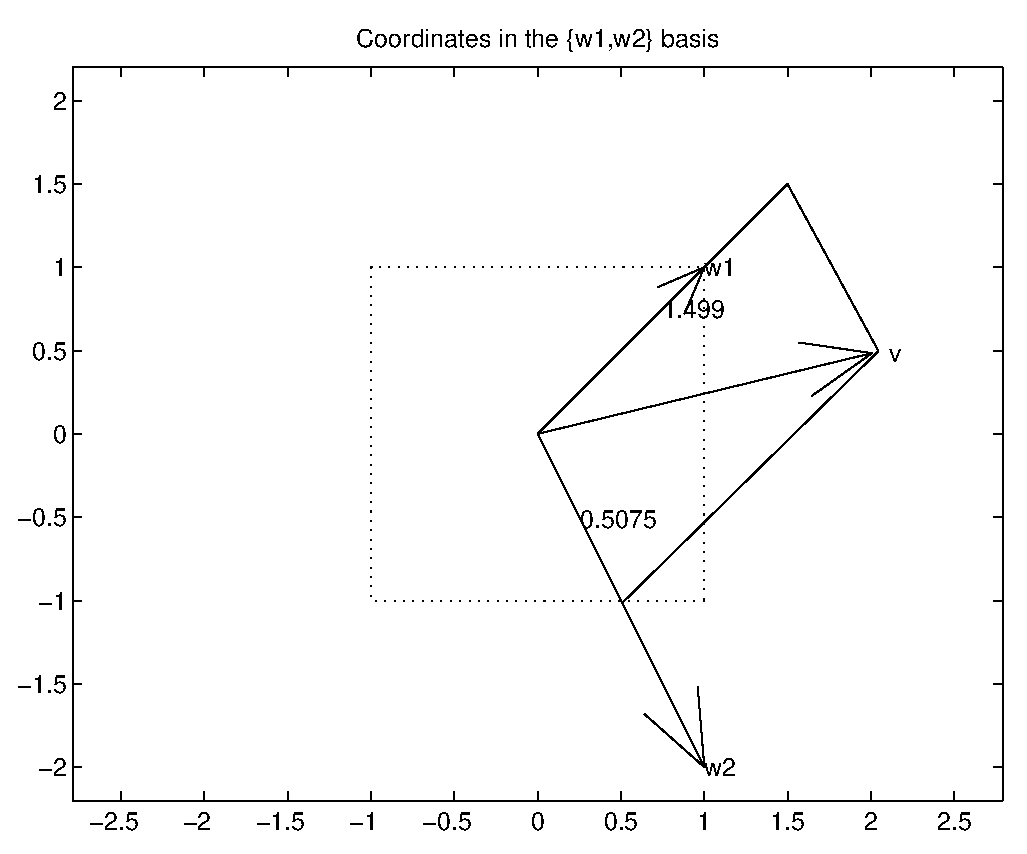
\psfig{file=figures/coord.eps,width=3.5in}}
     \caption{The coordinates of $v=(2.0,0.5)$ in the basis
	$w_1=(1,1), w_2=(1,-2)$.}
     \label{F:coords}
\end{figure}

\subsubsection*{Abstracting $\R^2$ to $\R^n$}
\index{coordinates!in ${\bf R}^n$}

Suppose that we are given a basis ${\cal W} = \{w_1,\ldots,w_n\}$ of
$\R^n$ and a vector $v\in\R^n$.  How do we find the coordinates
$[v]_{\cal W}$ of $v$ in the basis ${\cal W}$?

For definiteness, assume that $v$ and the $w_j$ are row vectors.  Equation
\Ref{e:coordv} may be rewritten as
\[
v^t = (w_1^t|\cdots|w_n^t)\vect{\alpha}{n}.
\]
Thus,
\begin{equation}  \label{e:coordRn}
[v]_{\cal W} = \vect{\alpha}{n} = P_{\cal W}\inv v^t,
\end{equation}
where $P_{\cal W} = (w_1^t|\cdots|w_n^t)$.  Since the $w_j$ are a basis for
$\R^n$, the columns of the matrix $P_{\cal W}$ are linearly independent, and
$P_{\cal W}$ is invertible.


We may use \Ref{e:coordRn} to compute $[v]_{\cal W}$ using
\Matlabp.  For example, let
\[
v  =  (4,1,3)
\]
and
\[
w_1 =  (1,4,7) \quad w_2 = (2,1,0) \quad w_3 = (-4,2,1).
\]
Then $[v]_{\cal W}$ is found by typing
\begin{verbatim}
w1 = [ 1 4 7];
w2 = [ 2 1 0];
w3 = [-4 2 1];
inv([w1' w2' w3'])*[4 1 3]'
\end{verbatim} \index{\computer!inv}  \index{\computer!'}
The answer is:

\begin{verbatim}
ans =
    0.5306
    0.3061
   -0.7143
\end{verbatim}


\subsection*{Determining the Matrix of a Linear Mapping in Coordinates}

Suppose that we are given the linear map $L_A:\R^n\to\R^n$ associated to
the matrix $A$ in standard coordinates and a basis $w_1,\ldots,w_n$ of $\R^n$.
How do we find the matrix $[L_A]_{\cal W}$. As above, we assume that the
vectors $w_j$ and the vector $v$ are row vectors  Since $L_A(v)=Av^t$ we can
rewrite \Ref{e:matrixofL} as
\[
[L_A]_{\cal W}[v]_{\cal W} = [Av^t]_{\cal W}
\]
As above, let $P_{\cal W}=(w_1^t|\cdots|w_n^t)$.  Using \Ref{e:coordRn} we
see that
\[
[L_A]_{\cal W}P_{\cal W}\inv v^t = P_{\cal W}\inv Av^t.
\]
Setting
\[
u= P_{\cal W}\inv v^t
\]
we see that
\[
[L_A]_{\cal W}u = P_{\cal W}\inv A P_{\cal W}u.
\]
Therefore,
\[
[L_A]_{\cal W} = P_{\cal W}\inv AP_{\cal W}.
\]
We have proved:
\begin{thm}
Let $A$ be an $n\times n$ matrix and let $L_A:\R^n\to\R^n$ be the associated
linear map.  Let ${\cal W} = \{w_1,\ldots,w_n\}$ be a basis\index{basis} for
$\R^n$.  Then the matrix $[L_A]_{\cal W}$ associated to to $L_A$ in the basis
${\cal W}$ is similar\index{similar} to $A$.  Therefore the determinant, trace,
and eigenvalues of $[L_A]_{\cal W}$ are identical to those of $A$.
\end{thm}




\subsection*{Matrix Normal Forms in $\R^2$} \index{normal form}

If we are careful about how we choose the basis ${\cal W}$, then
we can simplify the form of the matrix $[L]_{\cal W}$.  Indeed, we
have already seen examples of this process when we discussed how
to find closed form solutions to linear planar systems of ODEs in
the previous chapter.  For example, suppose that $L:\R^2\to\R^2$
has real eigenvalues $\lambda_1$ and $\lambda_2$ with two
linearly independent eigenvectors $w_1$ and $w_2$.  Then the
matrix associated to $L$ in the basis ${\cal W} = \{w_1,w_2\}$
is the diagonal matrix
\begin{equation}   \label{e:diagcoord}
[L]_{\cal W} = \mattwo{\lambda_1}{0}{0}{\lambda_2},
\end{equation}
since
\[
[L(w_1)]_{\cal W} = [\lambda_1w_1]_{\cal W} = \vectwo{\lambda_1}{0} \AND
[L(w_2)]_{\cal W} = [\lambda_2w_2]_{\cal W} = \vectwo{0}{\lambda_2}.
\]

In Chapter~\ref{Chap:Planar} we showed how to classify $2\times 2$
matrices up to similarity (see Chapter~\ref{Chap:Planar},
Theorem~\ref{T:putinform}) and how to use this classification to find
closed form solutions to planar systems of linear ODEs (see
Section~\ref{S:6.5}).  We now use
the ideas of coordinates and matrices associated with bases to
reinterpret the normal form result (Chapter~\ref{Chap:Planar},
Theorem~\ref{T:putinform}) in a more geometric fashion.

\begin{thm}  \label{T:putinform2}
Let $L:\R^2\to\R^2$ be a linear mapping.  Then in an appropriate
coordinate system defined by the basis ${\cal W}$ below, the matrix
$L_{\cal W}$ has one of the following forms.
\begin{itemize}
\item[(a)]	Suppose that $L$ has two linearly independent
real eigenvectors $w_1$ and $w_2$ with real eigenvalues $\lambda_1$
and $\lambda_2$.  Then
\[
[L]_{\cal W} = \mattwo{\lambda_1}{0}{0}{\lambda_2}.
\]

\item[(b)]	Suppose that $L$ has no real eigenvectors and
complex conjugate eigenvalues $\sigma\pm i\tau$ where
$\tau\neq 0$.  Let $w_1+iw_2$ be a complex eigenvector of $L$
associated with the eigenvalue $\sigma-i\tau$.
Then ${\cal W}=\{w_1,w_2\}$ is a basis and
\[
[L]_{\cal W} = \mattwo{\sigma}{-\tau}{\tau}{\sigma}.
\]

\item[(c)]	Suppose that $L$ has exactly one linearly
independent real eigenvector $w_1$ with real eigenvalue $\lambda$.
Choose the generalized eigenvector\index{eigenvector!generalized} $w_2$
\begin{equation}  \label{e:Lw=lw+v}
(L-\lambda I_2)(w_2) =  w_1.
\end{equation}
Then ${\cal W}=\{w_1,w_2\}$ is a basis and
\[
[L]_{\cal W} = \mattwo{\lambda}{1}{0}{\lambda}.
\]
\end{itemize}
\end{thm}

\begin{proof}
The verification of (a) was discussed in \Ref{e:diagcoord}.  The
verification of (b) follows from Chapter~\ref{Chap:Planar},
\Ref{e:complexcoord} on equating $w_1$ with $v$ and $w_2$ with $w$.
The verification of (c) follows directly from \Ref{e:Lw=lw+v} as
\[
[L(w_1)]_{\cal W} = \lambda e_1 \AND [L(w_2)]_{\cal W} = e_1+\lambda e_2.
\]
\end{proof}



\subsubsection*{Visualization of Coordinate Changes in ODEs}
\index{change of coordinates}

We consider two examples.  As a first example note that the matrices
\[
C = \mattwo{1}{0}{0}{-2} \AND B = \mattwo{4}{-3}{6}{-5},
\]
are similar matrices.   Indeed, $B = P\inv CP$ where
\begin{equation}  \label{e:Pchange}
P = \mattwo{2}{-1}{1}{-1}.
\end{equation}
The phase portraits of the differential equations $\dot{X}=BX$ and
$\dot{X}=CX$ are shown in Figure~\ref{F:comparesim}.  Note that both
phase portraits are pictures of the {\em same\/} saddle\index{saddle} ---
just in different coordinate systems\index{coordinate system}.

\begin{figure}[htb]
        \centerline{%
        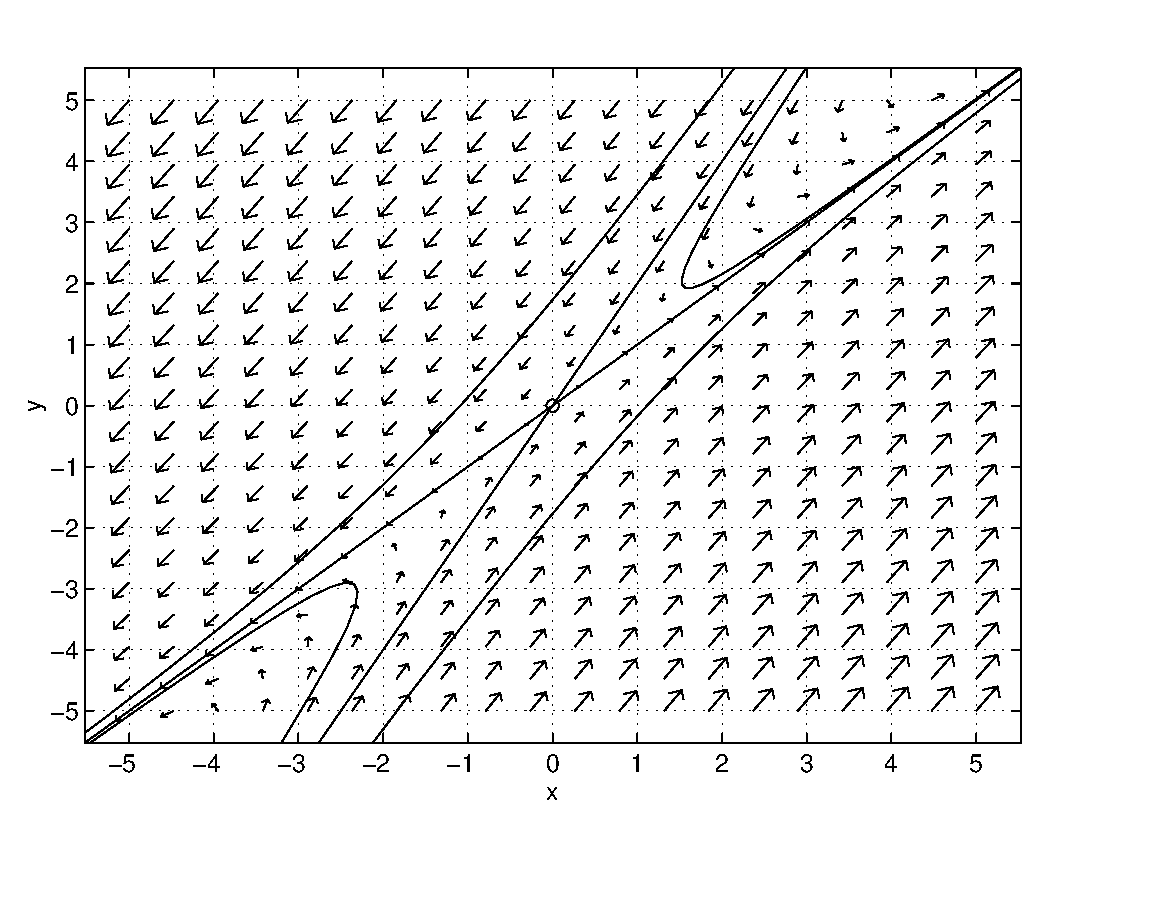
\psfig{file=figures/saddle7a.eps,width=3.2in}
        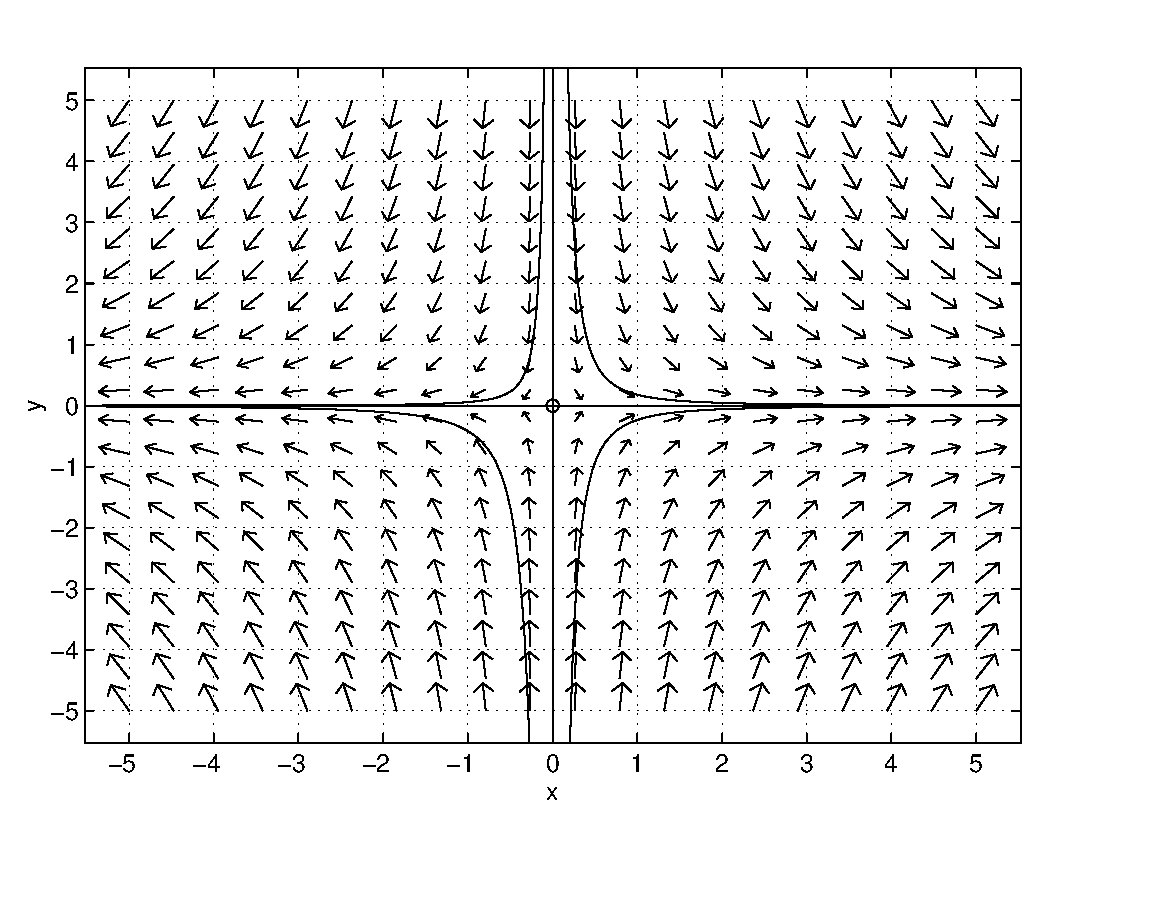
\psfig{file=figures/saddle7b.eps,width=3.2in}}
        \caption{Phase planes for the saddles $\dot{X}=BX$ and $\dot{X}=CX$.}
        \label{F:comparesim}
\end{figure}

As a second example note that the matrices
\[
C = \mattwo{0}{2}{-2}{0} \AND B = \mattwo{6}{-4}{10}{-6}
\]
are similar matrices, and both are centers.   Indeed, $B = P\inv CP$
where $P$ is the same matrix as in \Ref{e:Pchange}.  The phase portraits
of the differential equations $\dot{X}=BX$ and $\dot{X}=CX$ are shown in
Figure~\ref{F:comparesim2}.  Note that both phase portraits are pictures
of the {\em same\/} center\index{center} --- just in different coordinate
systems.



\begin{figure}[htb]
        \centerline{%
        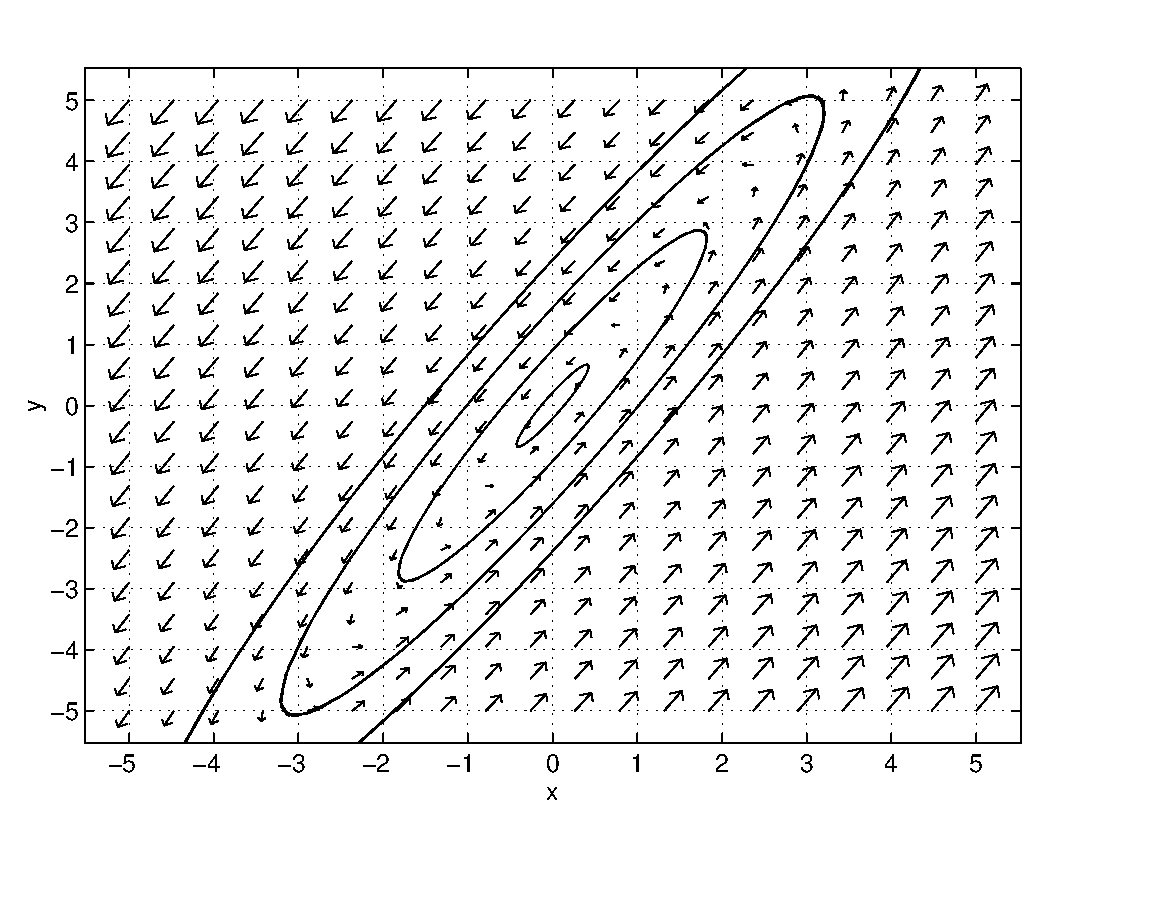
\psfig{file=figures/center7a.eps,width=3.2in}
        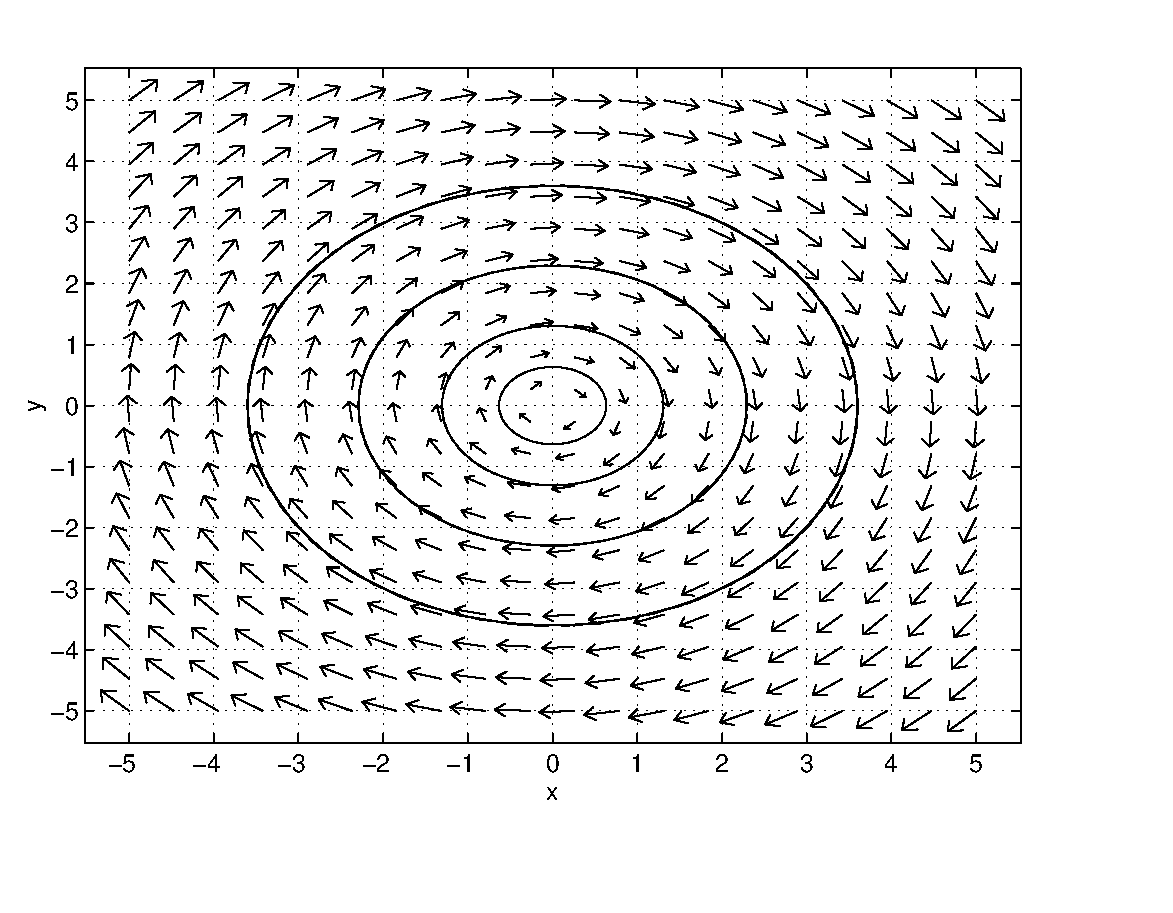
\psfig{file=figures/center7b.eps,width=3.2in}}
        \caption{Phase planes for the centers $\dot{X}=BX$ and $\dot{X}=CX$.}
        \label{F:comparesim2}
\end{figure}






\EXER

\TEXER

\begin{exercise} \label{c7.1.1}
Let
\[
w_1 = (1,4) \AND w_2 = (-2,1).
\]
Find the coordinates of $v=(-1,32)$ in the ${\cal W}$ basis.
\end{exercise}

\begin{exercise} \label{c7.3.1}
Let $w_1=(1,2)$ and $w_2=(0,1)$ be a basis for $\R^2$.  Let
$L_A:\R^2\to\R^2$ be the linear map given by the matrix
\[
A=\mattwo{2}{1}{-1}{0}
\]
in standard coordinates.  Find the matrix $[L]_{\cal W}$.
\end{exercise}

\begin{exercise} \label{c7.1.3}
Let $E_{ij}$ be the $2\times 3$ matrix whose entry in the
$i^{th}$ row and $j^{th}$ column is $1$ and all of whose
other entries are $0$.
\begin{itemize}
\item[(a)]  Show that
\[
{\cal V}=\{E_{11},E_{12},E_{13},E_{21},E_{22},E_{23}\}
\]
is a basis for the vector space of $2\times 3$ matrices.
\item[(b)]   Compute $[A]_{\cal V}$ where
\[
A=\left(\begin{array}{rrr} -1 & 0 & 2\\ 3 & -2 & 4\end{array}\right).
\]
\end{itemize}
\end{exercise}

\begin{exercise} \label{c7.1.4}
Verify that ${\cal V}= \{p_1,p_2,p_3\}$ where
\[
p_1(t)=1+2t, \quad p_2(t)=t+2t^2, \AND p_3(t)=2-t^2,
\]
is a basis for the vector space of polynomials ${\cal P}_2$.
Let $p(t)=t$ and find $[p]_{\cal V}$.
\end{exercise}

\CEXER


\begin{exercise} \label{c7.1.6}
Let
\[
w_1=(1,0,2), \quad w_2=(2,1,4), \AND w_3=(0,1,-1)
\]
be a basis for $\R^3$.  Find $[v]_{\cal W}$ where $v=(2,1,5)$.
\end{exercise}

\begin{exercise} \label{c7.1.7}
Let
\begin{equation*}
\begin{array}{ccl}
w_1 & = & (0.2,-1.3,0.34,-1.1)\\
w_2 & = & (0.5,-0.6,0.7,0.8)\\
w_3 & = & (-1.0,1.0,2.0,4.5) \\
w_4 & = & (-5.1,0.0,1.6,-1.7) \end{array}
\end{equation*}
be a basis ${\cal W}$ for $\R^4$.  Find $[v]_{\cal W}$ where
$v=(1.7,2.3,1.0,-5.0)$.
\end{exercise}

\begin{exercise} \label{c7.3.4}
Find a basis ${\cal W}=\{w_1,w_2\}$ such that $[L_A]_{\cal W}$ is
a diagonal matrix, where $L_A$ is the linear map associated with the
matrix
\[
A = \mattwo{-10}{-6}{18}{11}.
\]
\end{exercise}

\begin{exercise} \label{c7.3.5}
Let $A$ be the $4\times 4$ matrix
\begin{equation*}
A = \left( \begin{array}{rrrr}
    2   &  1   &   4   &   6\\
     1  &    2   &   1  &    1\\
     0   &   1    &  2   &   4\\
     2    &  1   &   1   &   5
\end{array}\right)
\end{equation*}
and let ${\cal W}=\{w_1,w_2,w_3,w_4\}$ where
\begin{equation*}
\begin{array}{rcl}
w_1 & = &  ( 1, 2, 3, 4)  \\
w_2 & = &  ( 0,-1, 1, 3) \\
w_3 & = &  ( 2, 0, 0, 1) \\
w_4 & = &   (-1, 1,3, 0)
\end{array}
\end{equation*}
Verify that ${\cal W}$ is a basis of $\R^4$ and compute the
matrix associated to $A$ in the ${\cal W}$ basis.
\end{exercise}




\section{Matrices of Linear Maps on a Vector Space}  \label{MALT}
\index{linear}  \index{coordinates}


Returning to the general finite dimensional vector space $V$, suppose that
\[
{\cal W} = \{w_1,\ldots,w_n\} \AND {\cal Z} = \{z_1,\ldots,z_n\}
\]
are bases of $V$.  Then we can write
\[
v = \alpha_1 w_1 + \cdots + \alpha_n w_n \AND
v = \beta_1 z_1 + \cdots + \beta_n z_n
\]
to obtain the coordinates
\begin{equation}  \label{e:vincoords}
[v]_{\cal W} = (\alpha_1,\ldots,\alpha_n) \AND
[v]_{\cal Z} = (\beta_1,\ldots,\beta_n)
\end{equation}
of $v$ relative to the bases ${\cal W}$ and ${\cal Z}$.  The question that
we address is: How are $[v]_{\cal W}$ and $[v]_{\cal Z}$ related?  We answer
this question by finding an $n\times n$ matrix $C_{{\cal W}{\cal Z}}$ such that
\begin{equation} \label{e:coordchange}
\vect{\alpha}{n} = C_{{\cal W}{\cal Z}} \vect{\beta}{n}.
\end{equation}
We may rewrite \Ref{e:coordchange} as
\begin{equation}  \label{e:coordchange2}
[v]_{\cal W} = C_{{\cal W}{\cal Z}}[v]_{\cal Z}.
\end{equation}

\begin{Def}
Let ${\cal W}$ and ${\cal Z}$ be bases\index{basis} for the $n$-dimensional
vector space $V$.  The $n\times n$ matrix $C_{{\cal W}{\cal Z}}$
is a {\em transition\/} matrix if $C_{{\cal W}{\cal Z}}$ satisfies
\Ref{e:coordchange2}.
\end{Def}  \index{matrix!transition}


\subsubsection*{Transition Mappings Defined}

The next theorem presents a method for finding the transition matrix
between coordinates associated to bases in an $n$-dimensional vector
space $V$.

\begin{thm}  \label{T:coordform}
Let ${\cal W}=\{w_1,\ldots,w_n\}$ and ${\cal Z}=\{z_1,\ldots,z_n\}$
be bases for the $n$-dimensional vector space\index{vector!space} $V$.
Then
\begin{equation} \label{e:coordform}
C_{{\cal W}{\cal Z}} =
\left(\begin{array}{ccc} c_{11} & \cdots & c_{1n} \\
\vdots & \vdots & \vdots \\
c_{n1} & \cdots & c_{nn} \end{array}\right)
\end{equation}
is the transition matrix, where
\begin{equation} \label{e:wtoz}
\begin{array}{ccc}
z_1 & = & c_{11}w_1 + \cdots + c_{n1}w_n \nonumber \\
    & \vdots &  \\
z_n & = & c_{1n}w_1 + \cdots + c_{nn}w_n \nonumber
\end{array}
\end{equation}
for scalars $c_{ij}$.
\end{thm}

\begin{proof}
We can restate \Ref{e:wtoz} as
\[
[z_j]_{\cal W} = \left(\begin{array}{c} c_{1j} \\ \vdots \\c_{nj}
\end{array} \right).
\]
Note that
\[
[z_j]_{\cal Z} = e_j,
\]
by definition.  Since the transition matrix satisfies
$[v]_{\cal W} =  C_{{\cal W}{\cal Z}}[v]_{\cal Z}$ for all vectors
$v\in V$, it must satisfy this relation for $v=z_j$.  Therefore,
\[
[z_j]_{\cal W} = C_{{\cal W}{\cal Z}}[z_j]_{\cal Z} = C_{{\cal W}{\cal Z}}e_j.
\]
It follows that $[z_j]_{\cal W}$ is the $j^{th}$ column of
$C_{{\cal W}{\cal Z}}$, which proves the theorem.  \end{proof}

\subsubsection*{A Formula for $C_{\cal WZ}$ when $V=\R^n$}

For bases in $\R^n$, there is a formula for finding transition
matrices\index{matrix!transition}.  Let ${\cal W} =\{w_1,\ldots,w_n\}$
and ${\cal Z} = \{z_1,\ldots,z_n\}$ be bases of $\R^n$ --- written as row
vectors.
Also, let $v\in\R^n$ be written as a row vector.  Then \Ref{e:coordRn}
implies that
\[
[v]_{\cal W} = P_{\cal W}\inv v^t \AND [v]_{\cal Z} = P_{\cal Z}\inv v^t,
\]
where
\[
P_{\cal W} = (w_1^t|\cdots|w_n^t) \AND  P_{\cal Z} = (z_1^t|\cdots|z_n^t).
\]
It follows that
\[
[v]_{\cal W} = P_{\cal W}\inv P_{\cal Z} [v]_{\cal Z}
\]
and that
\begin{equation} \label{e:coordformn}
C_{\cal WZ} = P_{\cal W}\inv P_{\cal Z}.
\end{equation}

As an example, consider the following bases of $\R^4$.  Let
\begin{equation*}
\begin{array}{ccccccc}
w_1 & = & [1, 4, 2, 3] & \hspace{0.2in} & z_1 & = & [3, 2, 0, 1] \\
w_2 & = & [2, 1, 1, 4] &  		    & z_2 & = & [-1, 0, 2, 3] \\
w_3 & = & [0, 1, 5, 6] & 		    & z_3 & = & [3, 1, 1, 3] \\
w_4 & = & [2, 5, -1, 0] & 		    & z_4 & = & [2, 2, 3, 5]
\end{array}
\end{equation*}
Then the matrix $C_{\cal WZ}$ is obtained by typing {\tt e9\_4\_7} to
enter the bases and
\begin{verbatim}
inv([w1' w2' w3' w4'])*[z1' z2' z3' z4']
\end{verbatim}
to compute $C_{\cal WZ}$.  The answer is:
\begin{verbatim}
ans =
   -8.0000    5.5000   -7.0000   -3.2500
   -0.5000    0.7500    0.0000    0.1250
    4.5000   -2.7500    4.0000    2.3750
    6.0000   -4.0000    5.0000    2.5000
\end{verbatim}



\subsubsection*{Coordinates Relative to Two Different Bases in $\R^2$}

Recall the basis ${\cal W}$
\[
w_1=(1,1) \AND w_2=(1,-2)
\]
of $\R^2$ that was used in a previous example.  Suppose that
${\cal Z}=\{z_1,z_2\}$ is a second basis of $\R^2$.  Write $v=(v_1,v_2)$
as a linear combination of the basis ${\cal Z}$
\[
v=\beta_1z_1 + \beta_2z_2,
\]
obtaining the coordinates $[v]_{\cal Z}=(\beta_1,\beta_2)$.

We use \Matlab to illustrate how the coordinates of a vector $v$ relative
to two bases may be viewed geometrically.  Suppose that $z_1=(1,3)$ and
$z_2=(1,-2)$.  Then enter the two bases ${\cal W}$ and ${\cal Z}$ by typing
\begin{verbatim}
w1 = [1 1];
w2 = [1 -2];
z1 = [1 3];
z2 = [-1 2];
ccoord
\end{verbatim}


The \Matlab program {\sf ccoord}\index{\computer!ccoord} opens two
graphics windows
representing the ${\cal W}$ and ${\cal Z}$ planes with the basis
vectors plotted in red.  Clicking the left mouse button on a
vector in the ${\cal W}$ plane simultaneously plots this vector
$v$ in both planes in yellow and the coordinates of $v$ in the
respective bases in cyan.  See Figure~\ref{F:2coords}.  From
this display you can visualize the coordinates of a
vector relative to two different bases.

\begin{figure}[htb]
     \centerline{%
     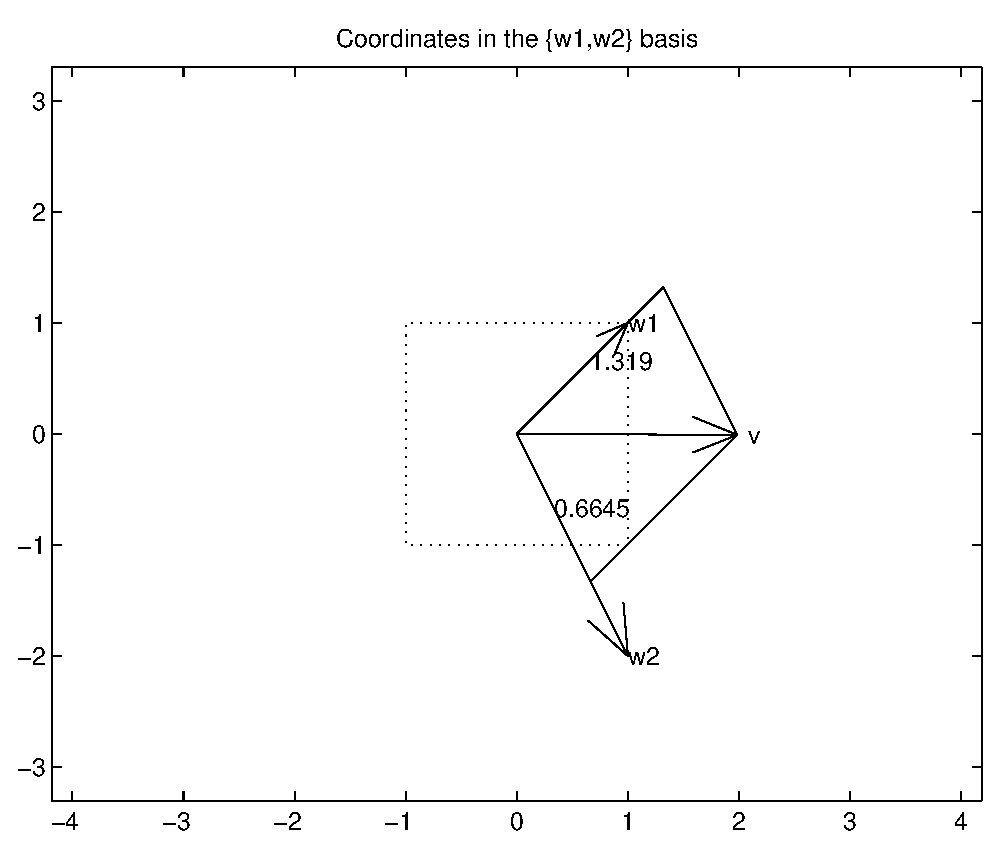
\psfig{file=figures/ccoorda.eps,width=3.0in}
	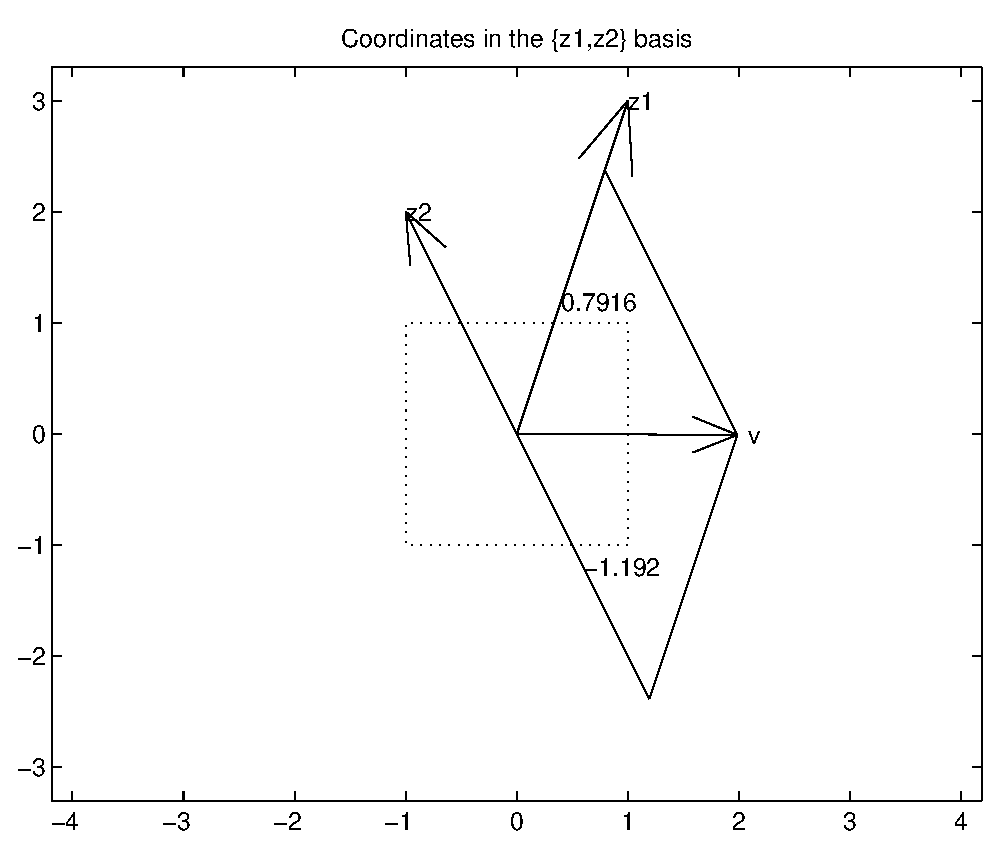
\psfig{file=figures/ccoordb.eps,width=3.0in}}
     \caption{The coordinates of $v=(1.9839,-0.0097)$ in the bases
	$w_1=(1,1), w_2=(1,-2)$ and $z_1=(1,3),z_2=(-1,2)$.}
     \label{F:2coords}
\end{figure}

Note that the program {\sf ccoord} prints the transition matrix
$C_{\cal WZ}$ in the \Matlab control window.  We can verify the
calculations of the program {\sf ccoord} on this example by hand.
Recall that \Ref{e:coordformn} states that
\begin{eqnarray*}
C_{\cal WZ} & = & \mattwo{1}{2}{2}{3}\inv\mattwo{1}{2}{4}{1} \\
& = & \mattwo{-3}{2}{2}{-1}\mattwo{1}{2}{4}{1} \\
& = & \mattwo{5}{-4}{-2}{3}.
\end{eqnarray*}


\subsection*{Matrices of Linear Maps in Different Bases}

\begin{thm} \label{T:matrixcoord}
Let $L:V\to V$ be a linear mapping\index{linear!mapping} and let
${\cal W}$ and ${\cal Z}$ be bases of $V$.  Then
\[
[L]_{\cal Z} \AND [L]_{\cal W}
\]
are similar \index{similar} matrices.  More precisely,
\begin{equation}  \label{e:matrixcoord}
[L]_{\cal W} = C_{{\cal Z}{\cal W}}\inv [L]_{\cal Z} C_{{\cal Z}{\cal W}}.
\end{equation}
\end{thm}

\begin{proof}  For every $v\in\R^n$ we compute
\begin{eqnarray*}
C_{{\cal Z}{\cal W}}[L]_{\cal W}[v]_{\cal W} & = &
C_{{\cal Z}{\cal W}}[L(v)]_{\cal W} \\
& = & [L(v)]_{\cal Z}  \\
& = & [L]_{\cal Z}[v]_{\cal Z} \\
& = & [L]_{\cal Z} C_{{\cal Z}{\cal W}}[v]_{\cal W}.
\end{eqnarray*}
Since this computation holds for every $[v]_{\cal W}$, it follows that
\[
C_{{\cal Z}{\cal W}}[L]_{\cal W} = [L]_{\cal Z} C_{{\cal Z}{\cal W}}.
\]
Thus \Ref{e:matrixcoord} is valid.  \end{proof}





\EXER

\TEXER

\begin{exercise} \label{c7.1.2}
Let
\[
w_1 = (1,2) \AND w_2 = (0,1)
\]
and
\[
z_1 = (2,3) \AND z_2 = (3,4)
\]
be two bases of $\R^2$.  Find $C_{WZ}$.
\end{exercise}



\begin{exercise} \label{c7.3.2}
Let $f_1(t)=\cos t$ and $f_2(t)=\sin t$ be functions in $\CCone$.
Let $V$ be the two dimensional subspace spanned by $f_1,f_2$; so
${\cal F}=\{f_1,f_2\}$ is a basis for $V$.  Let $L:V\to V$ be the
linear mapping defined by $L(f)=\frac{df}{dt}$.  Find $[L]_{\cal F}$.
\end{exercise}

\begin{exercise} \label{c7.3.3}
Let $L:V\to W$ and $M:W\to V$ be linear mappings, and assume $\dim V > \dim W$.
Show that $M\compose L:V\to V$ is not invertible.
\end{exercise}

\CEXER

\begin{exercise} \label{c7.1.5}
Let
\[
w_1 = (0.23,0.56) \AND w_2 = (0.17,-0.71)
\]
and
\[
z_1 = (-1.4,0.3) \AND z_2 = (0.1,-0.2)
\]
be two bases of $\R^2$ and let $v=(0.6,0.1)$.  Find $[v]_{\cal
W}$, $[v]_{\cal Z}$, and $C_{\cal WZ}$.
\end{exercise}

\begin{exercise}  \label{c7.5.A}
Consider the matrix
\begin{equation*}
A = \frac{1}{3}\left(\begin{array}{ccc}
	1 & 1-\sqrt{3} & 1+\sqrt{3} \\
	1+\sqrt{3} & 1 & 1-\sqrt{3} \\
	1-\sqrt{3} & 1+\sqrt{3} & 1
	\end{array}\right)
  =  \left(\begin{array}{rrr}
    0.3333  & -0.2440  &  0.9107\\
    0.9107  &  0.3333  & -0.2440\\
   -0.2440  &  0.9107  &  0.3333
 \end{array}\right)
\end{equation*}
\begin{itemize}
\item[(a)]  Try to determine the way that the matrix $A$ moves vectors
in $\R^3$.  For example, let
\[
w_1=(1,1,1)^t \qquad w_2 = \frac{1}{\sqrt{6}}(1,-2,1)^t \qquad w_3 =
\frac{1}{\sqrt{2}}(1,0,-1)^t
\]
and compute $Aw_j$.
\item[(b)]  Let ${\cal W} = \{w_1,w_2,w_3\}$ be the basis of $\R^3$ given
in (a).  Compute $[L_A]_{\cal W}$.
\item[(c)]  Determine the way that the matrix $[L_A]_{\cal W}$ moves 
vectors in $\R^3$.  For example, consider how this matrix moves the standard 
basis vectors $e_1,e_2,e_3$.  Compare this answer with that in part (a).
\end{itemize}
\end{exercise}

\end{document}
